\chapter{Progettazione}
La fase di progettazione prevede principalmente la scelta dell'architettura da usare, su cui costruire il sistema. 
\\Per identificare l'architettura ideale bisogna elencare quali sono i componenti che ne fanno parte e in che modo sono interconnessi.
\begin{itemize}
	\item I componenti sono di due tipologie:
		\begin{itemize}
			\item Dispositivi utente, rappresentano i dispositivi fisici concessi ai dipendenti (smartphone o applicazione desktop)
			\item Sistema centrale, racchiude la logica di gestione e a cui i dispositivi utente possono fare accesso.
		\end{itemize}
	\item I connettori sono principalmente protocolli di rete, in quanto il sistema è pensato per dipendenti che hanno la possibilità di spostarsi all'interno del locale e accedere al sistema centra in modalità remota.
\end{itemize}
Alla base di ciò i componenti devono ricevere dei cambiamenti del sistema tramite opportune \textit{notifiche}, evitando quindi attese attive.

\section{Architettura}
Lo stile architetturale utilizzato per realizzare il sistema  è il \textbf{Publish-Subscribe}. Per la realizzazione dell'applicativo infatti vengono ripresi tutti i vantaggi dello stile a \textit{invocazione implicita}:
\begin{itemize}
	\item Tutti i componenti sono altamente disaccoppiati, favorendo la scalabilità del sistema. Il proprietario può quindi assumere/licenziare i dipendenti, o cambiarne i ruoli senza vincolarsi dal sistema.
	\item Tutta la comunicazione avviene tramite chiamate invocate implicitamente in risposta ad un evento.
\end{itemize}
In relazione ai componenti descritti, tutti i dipendenti sono dei \textit{Subscribers} mentre il sistema centrale è l'unico \textit{Publisher}.
\\I dipendenti, effettuando l'accesso, si iscrivono in automatico al Publisher.
Dato che il sistema può contenere un numero notevole di dipendenti, il Publisher fa uso di \textbf{Proxy} per smistare i messaggi solamente a specifici Subscibers.
\\Essi infatti all'atto del login non conoscono i Proxy del sistema, ma è il sistema stesso che li racchiude in gruppi (con lo stesso ruolo) e li associa a determinati Proxy.
\\Riassumendo quindi:
\begin{table}[H]
	\centering
	\begin{tabular}{|l | p{0.7\linewidth} |}
		\hline
		\textbf{Componenti} & Publisher, Subscribers, 
		Proxy \\
		\hline
		\textbf{Connettori} & Protocolli di rete \\
		\hline
		\textbf{Dati} & Notifiche \\
		\hline
		\textbf{Topologia} & Subscribers sono connessi al Publisher indirettamente, ricevendo e inviando notifiche attraverso i Proxy \\
		\hline
		\textbf{Vantaggi} & Subscribers sono tutti disaccoppiati lavorando in parallelo. Le notifiche vengono ben distribuite grazie ai Proxy \\
		\hline
		\textbf{Svantaggi} & Il controllo computazionale è caricato tutto sul sistema centrale. Nessuna conoscenza di quali componenti risponderanno ad un eventi \\
		\hline
	\end{tabular}
\end{table}


\subsection{Component Diagram}
\begin{figure}[H]
	\centering
	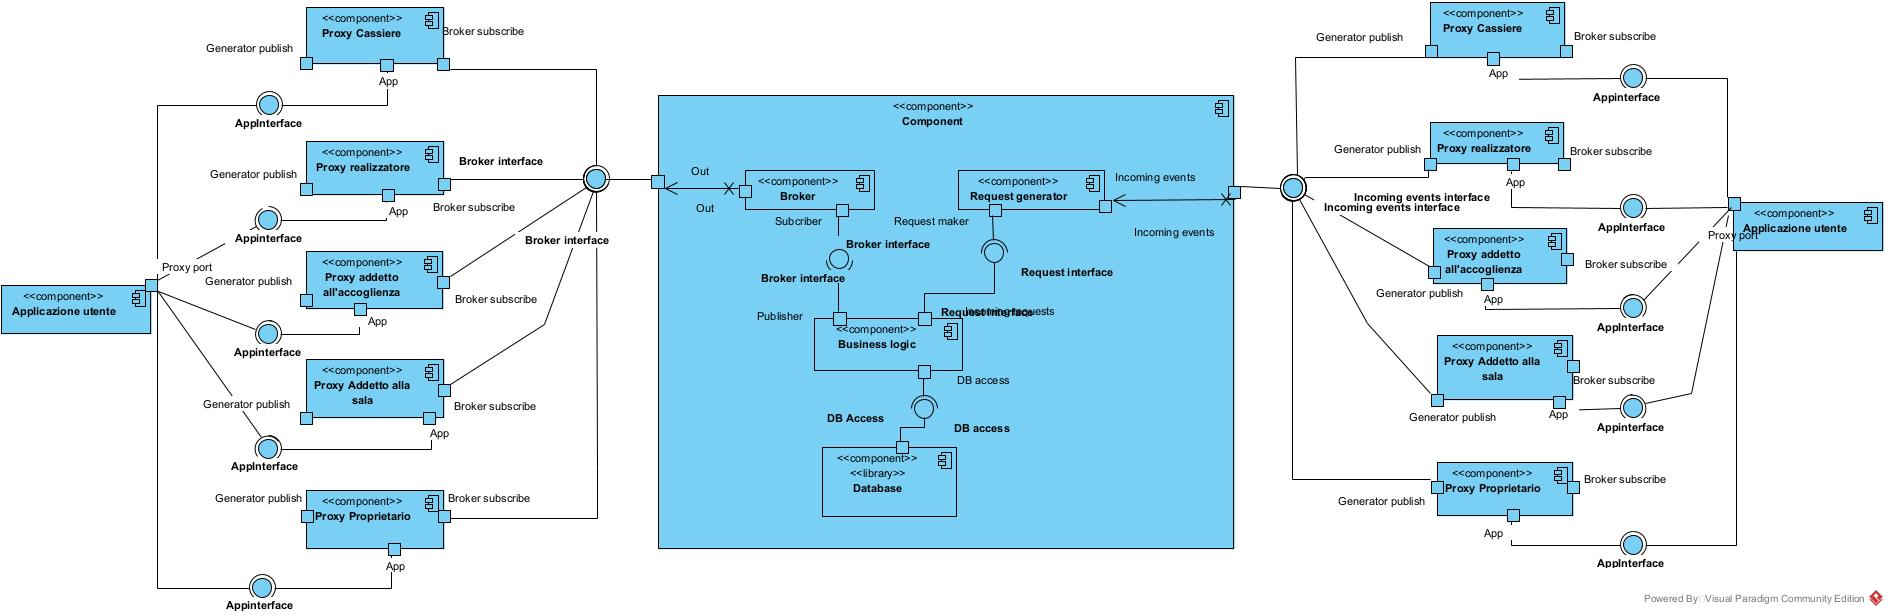
\includegraphics[width=1\textwidth]{Immagini/dynamic components.jpg}
\end{figure}

\section{Database}
Il database deve contenere le informazioni di base che devono essere utilizzate, a partire dai dipendenti che vengono registrati nel sistema e finire con le ordinazioni che vengono effettuate durante l'utilizzo del sistema.
\begin{figure}[H]
	\centering
	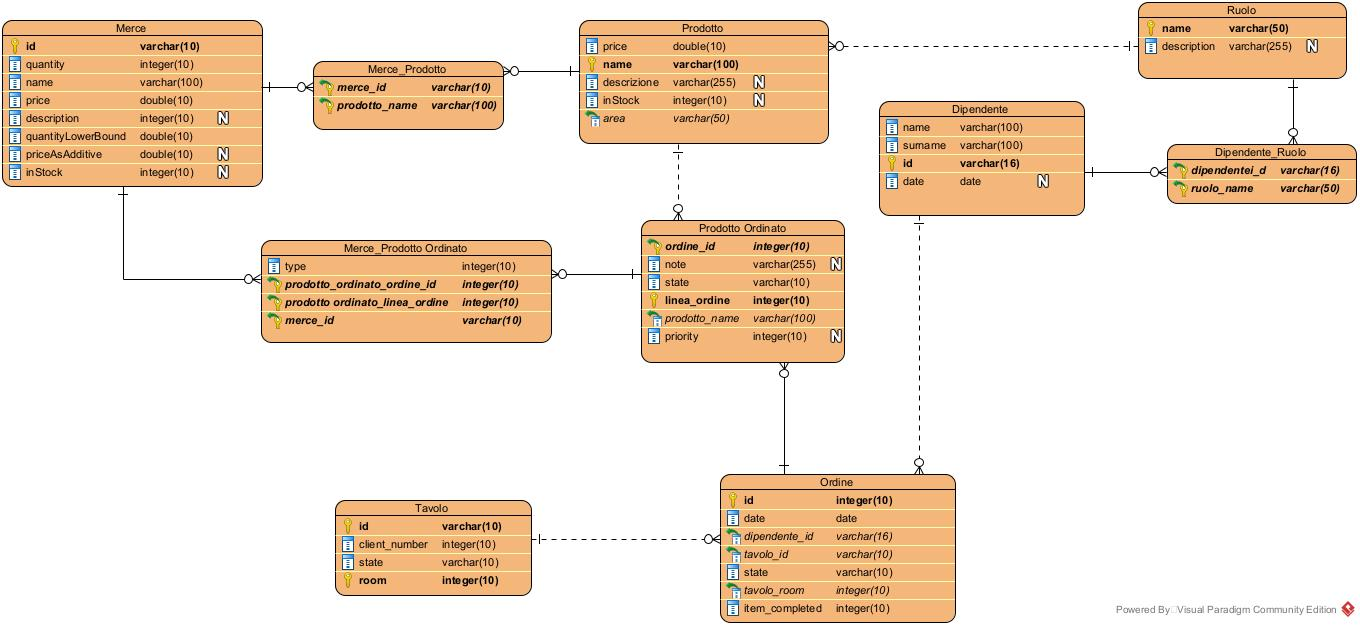
\includegraphics[width=1\textwidth]{Immagini/database.jpg}
\end{figure}
Le caratteristiche principali del database sono le seguenti:
\begin{enumerate}
	\item Le merci hanno, oltre alle informazioni di base quali prezzo, codice identificativo, nome, etc, hanno un attributo \textit{priceAsAdditive}. Tale attributo, se non nullo, indica il prezzo da aggiungere se quella merce è usata come merce aggiuntiva di un prodotto.
	\item Il \textit{Prodotto Ordinato} è un'associazione ternaria tra \textit{Ordine}, \textit{Prodotto} e \textit{Merce}.
	 \item Ogni prodotto ha un attributo collegato all'entità \textit{Ruoli}. Esso serve per indicare a che attività appartiene quel prodotto.
\end{enumerate}
Il precedente database si riferisce solo ai casi d'uso che si sono scelti di implementare. Non contiene, ad esempio, la gestione delle vendite e lo storico del locale.

\section{Deployment Diagram}
\section{Class Diagram}
\section{Sequence Diagram}